\documentclass[aspectratio=169]{beamer}
\usepackage{booktabs}
\usepackage{xcolor}
\usepackage{changepage}
\usepackage[export]{adjustbox}
\usepackage{booktabs}
\usepackage{graphbox}

\usetheme[numbering=fraction,progressbar=frametitle,sectionpage=none]{metropolis}


% Backup
\newcommand{\backupbegin}{%
   \newcounter{finalframe}
   \setcounter{finalframe}{\value{framenumber}}
}
\newcommand{\backupend}{%
   \setcounter{framenumber}{\value{finalframe}}
}


% Colors
\definecolor{myBlue}{RGB}{21, 56, 110}
\definecolor{myRed}{RGB}{174,0,34}
\definecolor{myRedBg}{RGB}{251, 217, 224}
\definecolor{greySAS}{RGB}{167,166,166}
\definecolor{greyCU}{RGB}{44,46,53}

\setbeamercolor{title}{fg=myBlue}
\setbeamercolor{background canvas}{bg=white}
\setbeamercolor{normal text}{fg=black}
\setbeamercolor{frametitle}{fg=myBlue, bg=white}
\setbeamercolor{section title}{fg=myBlue}
\setbeamercolor{title separator}{fg=myRed,bg=myRedBg}
\setbeamercolor{progress bar}{fg=myRed,bg=myRedBg}
\setbeamercolor{structure}{fg=myRed}


% Thicker progress bar
\makeatletter
\setlength{\metropolis@titleseparator@linewidth}{1pt}
\setlength{\metropolis@progressonsectionpage@linewidth}{1pt}
\setlength{\metropolis@progressinheadfoot@linewidth}{1pt}
\makeatother


% Commands
\newcommand{\bluetext}[1]{%
  \textcolor{myBlue}{#1}
}
\newcommand{\redtext}[1]{%
  \textcolor{myRed}{#1}
}


% Variables
\def\pt{\ensuremath{p_\mathrm{T}}}


% Title
\title[FCCcalo]{Calorimetry for Future Circular Collider}
\author[Faltova, Smiesko]{Jana~Faltov\'{a}\inst{1}, Juraj~Smie\v{s}ko\inst{1,2}}
\institute[CU, SAS]{\inst{1} Charles University, Czechia \\
                    \inst{2} Slovak Academy of Sciences, Slovakia}
\date[2021-May-19]{\footnotesize
                   IPNP Seminar, Prague \\
                   19 May 2020}
\titlegraphic{\vspace{6.1cm}\centering
\includegraphics[width=0.6\linewidth]{figures/logolink_OP_VVV_hor_barva_eng.jpg}}

%
% -----------------------------------------------------------------------------
%
\begin{document}

{%
  \setbeamercolor{background canvas}{bg=greyCU}
  \begin{frame}[noframenumbering]
    \centering
    \vspace{1cm}
    
\includegraphics[width=.25\textwidth]{figures/CU_red_white_logo.pdf}
    \thispagestyle{empty}
  \end{frame}
}

\begin{frame}
  \titlepage{}
  \thispagestyle{empty}
\end{frame}


\begin{frame}
  \frametitle{Overview}

  \tableofcontents
\end{frame}

%
% -----------------------------------------------------------------------------
%
\section{Future Circular Collider}

\begin{frame}
  \frametitle{Future Circular Collider}

  \begin{columns}[c]
    \column{.55\textwidth}

    \vspace*{1mm}
    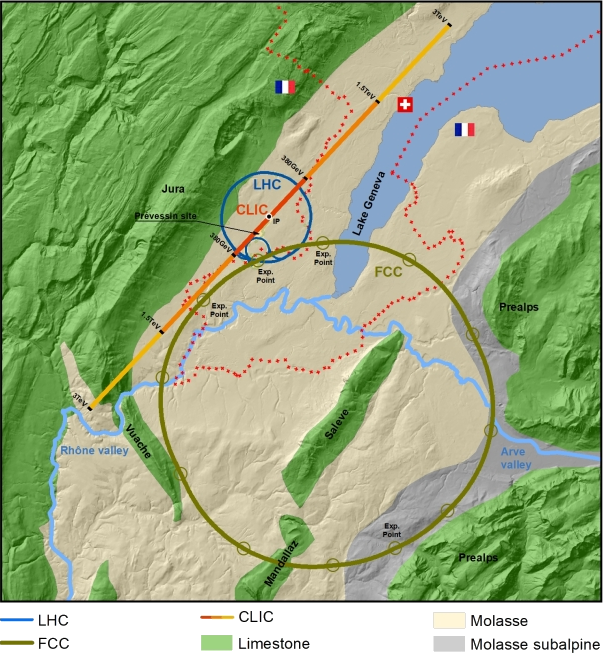
\includegraphics[width=0.9\linewidth]{figures/FCC_CLIC.png}\\[-1mm]
    \tiny{Image: \href{https://alumni.cern/news/226282}{CERN}}

    \column{.45\textwidth}
    \bluetext{European Particle Physics Strategy:}
    \begin{itemize}
      \item Investigate feasibility for FCC at CERN
      \item As global endeavor
    \end{itemize}

    \bluetext{FCC Plan:}
    \begin{itemize}
      \item Ring circumference 100 km
      \item Electron-positron collider as first step
      \item Hadron collider: $\sqrt{s} = 100$~TeV
    \end{itemize}
  \end{columns}
\end{frame}

\begin{frame}
  \frametitle{FCC-ee: Lepton Collider}

  \begin{columns}[c]
    \column{.5\textwidth}
    \begin{center}
      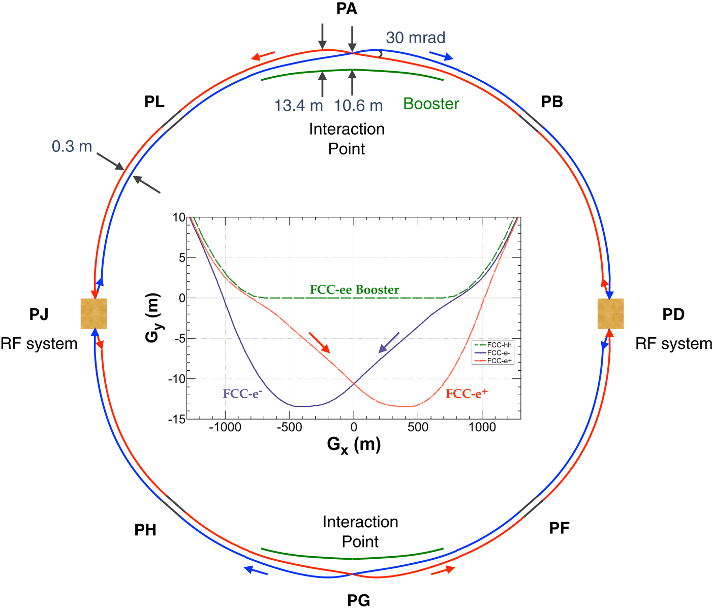
\includegraphics[width=.8\linewidth]{figures/FCC_ee_ring.png}
    \end{center}

    \vspace*{-1em}
    \bluetext{FCC-ee characteristics:}
    \begin{itemize}
      \item For precision physics
      \item Higgs factory
      \item EW precision increase by two digits
    \end{itemize}

    \column{.5\textwidth}
    \begin{center}
    {\footnotesize\hspace{3.3em}88--95
                  \hspace{0.2em}\textcolor{blue}{158--162}
                  \hspace{0.2em}\textcolor{red}{240
                  }\hspace{1.9em}\textcolor{green}{345--365} GeV}
      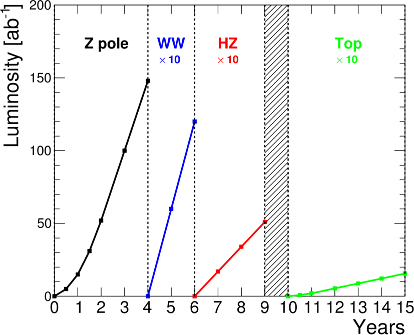
\includegraphics[width=.85\linewidth]{figures/FCC_ee_operation_plan.png}
    \end{center}

    \vspace*{-1em}
    \begin{itemize}
      \item Operation at four energies
      \item Clean environment
      \item ``Continuous'' beams
    \end{itemize}
  \end{columns}
\end{frame}

\begin{frame}
  \frametitle{FCC-hh: Hadron Collider}

  \begin{columns}[c]
    \column{.5\textwidth}
    \begin{center}
      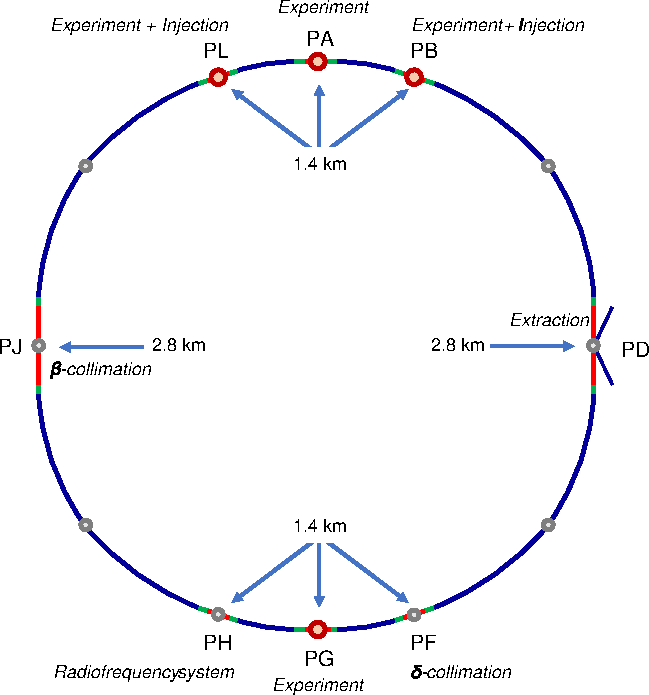
\includegraphics[width=.75\linewidth]{figures/FCC_hh_ring.pdf}
    \end{center}

    \bluetext{FCC-hh characteristics:}
    \begin{itemize}
      \item Continuation of energy frontier
    \end{itemize}

    \column{.5\textwidth}
    \begin{center}
      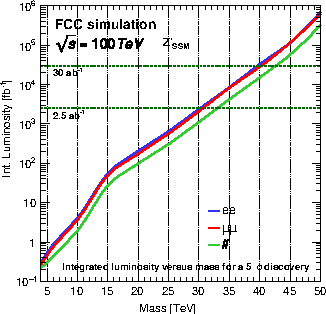
\includegraphics[width=.8\linewidth]{figures/FCC_hh_Zprime_ll.pdf}
    \end{center}

    \begin{itemize}
      \item Operation at 100~TeV energies
      \item 16~T magnets needed
    \end{itemize}
  \end{columns}
\end{frame}

%
% -----------------------------------------------------------------------------
%
\section{FCC Detectors}

\begin{frame}
  \frametitle{FCC-ee: CLD Detector}

  \begin{columns}[c]
    \column{.6\textwidth}
    \begin{center}
      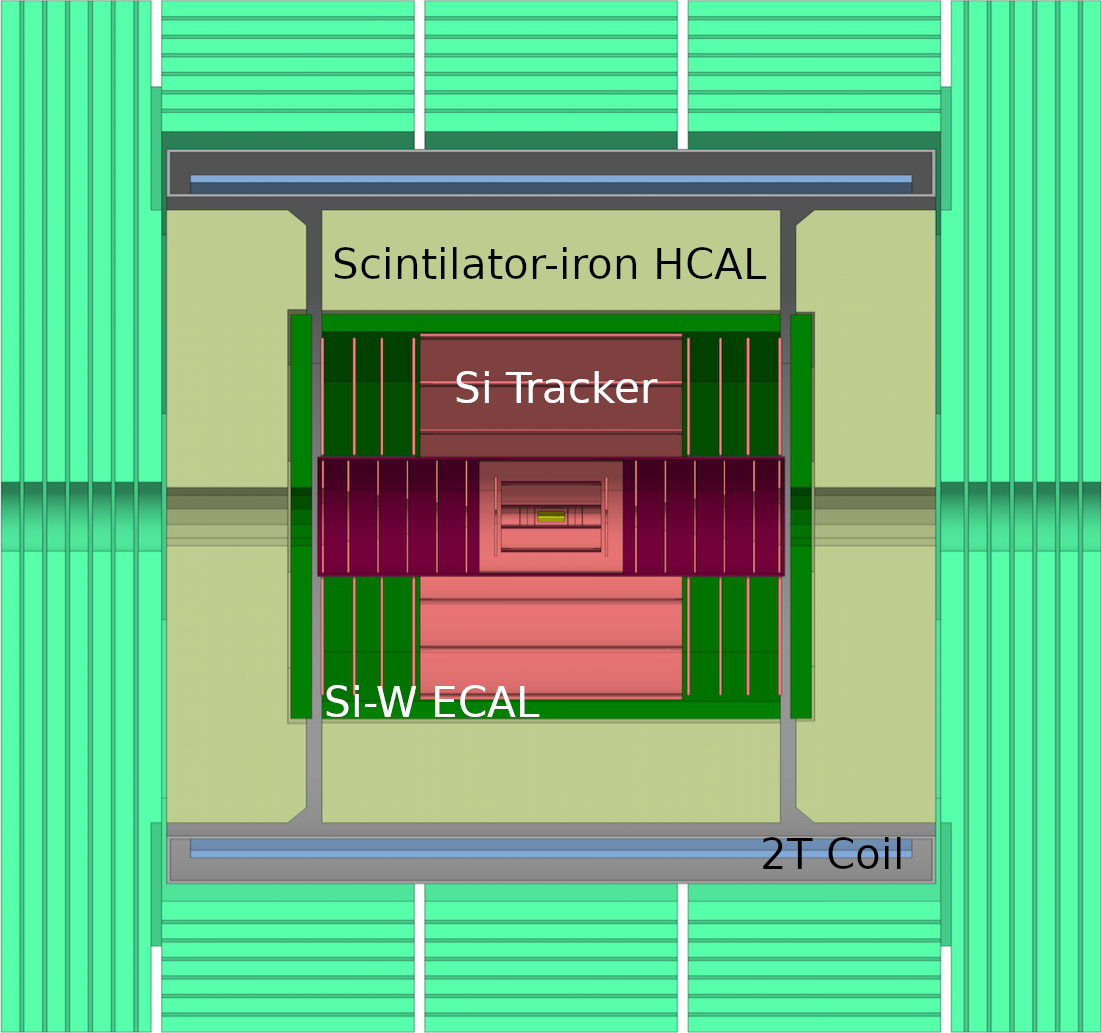
\includegraphics[width=0.9\linewidth]{figures/FCC_ee_CLD_text.png}
    \end{center}

    \column{.4\textwidth}
    \begin{itemize}
      \item Based on the detector for CLIC
      \item Silicon vertex detector and tracker
      \item 3D-imaging highly-granular calorimeter
      \item Coil outside calorimeter system
      \item Proved concept, understood performance
    \end{itemize}
  \end{columns}
\end{frame}

\begin{frame}
  \frametitle{FCC-ee: IDEA Detector}

  \begin{columns}[c]
    \column{.6\textwidth}
    \begin{center}
      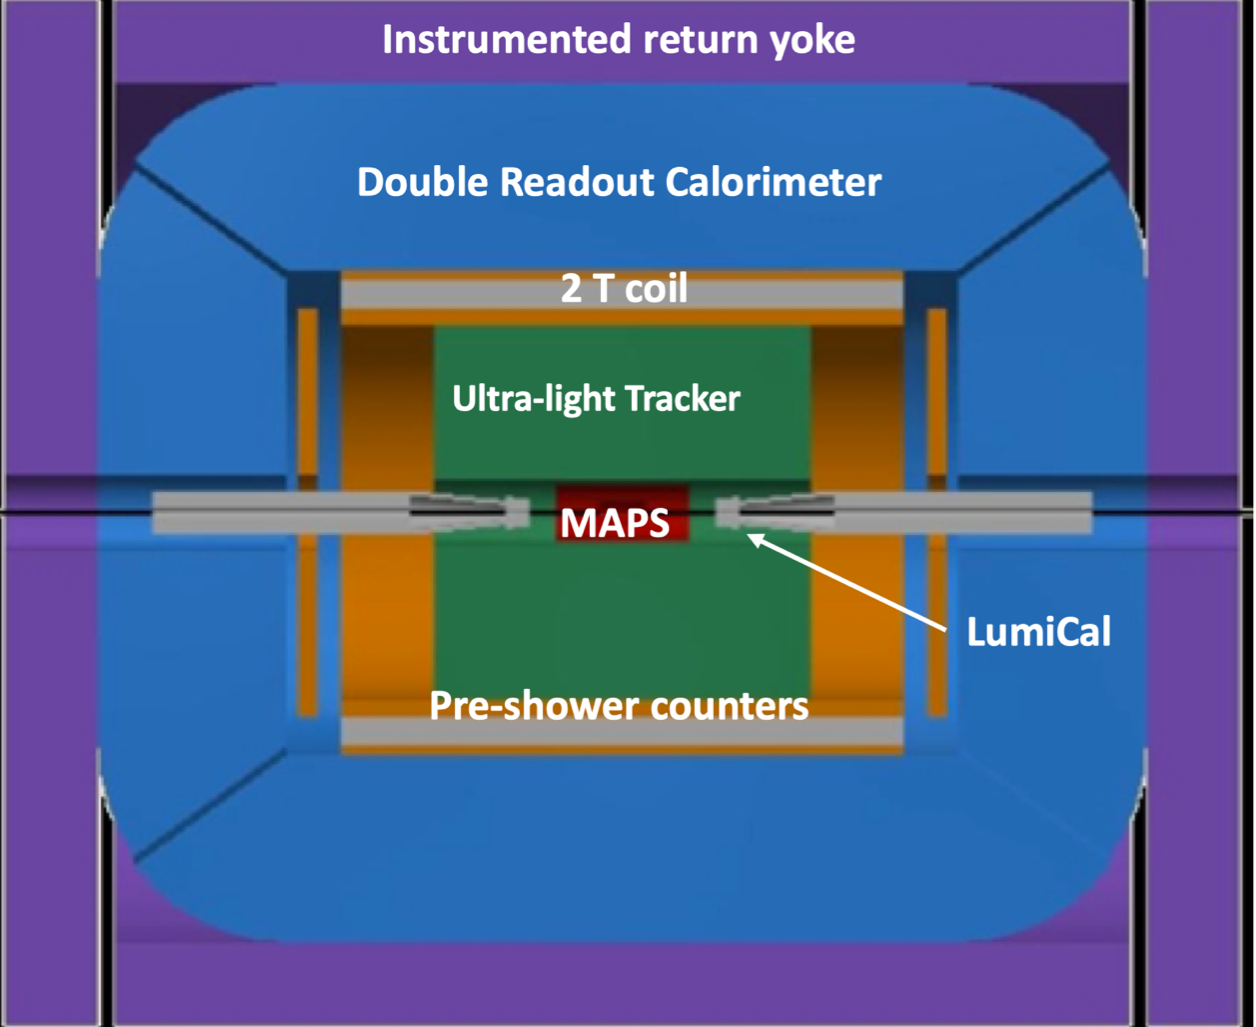
\includegraphics[width=\linewidth]{figures/FCC_ee_IDEA.png}
    \end{center}

    \column{.4\textwidth}
    \begin{itemize}
      \item New, innovative, possibly more cost-effective design
      \item Silicon vertex detector
      \item Short-drift, ultra-light wire chamber
      \item Dual-readout calorimeter
      \item Thin and light solenoid coil inside calorimeter system
    \end{itemize}
  \end{columns}
\end{frame}


%
% -----------------------------------------------------------------------------
%
\section{Noble Liquid Calorimetry for FCC-ee}

\begin{frame}
  \frametitle{FCC-ee Calorimetry}

  \vspace{2ex}
  \begin{columns}[c]
    \column{.5\textwidth}
    \bluetext{Requirements:}
    \begin{itemize}
      \item Jet-jet inv.\ mass resolution to resolve $W$ from $Z$
            \begin{itemize}
              \item requires $\sim 3$\% ($\sim 30\% / \sqrt{E}$\,)
            \end{itemize}
      \item EM resolution at minimum 15\% to sustain jet resolution\\[-0.4ex]
            \begin{itemize}
              \item $B_\text{S} \rightarrow D_\text{S}K$ requires $\sim 5$\%
            \end{itemize}
      \item Crystal and LAr --- good EM resolution
      \item CALICE and Dual Readout --- good jet resolution
    \end{itemize}

    \column{.5\textwidth}
    \bluetext{Energy resolution param.:}
    \[ \frac{\sigma_\text{E}}{\langle E\,\rangle} = \frac{a}{\sqrt{E\,}} \oplus
                                                    \frac{b}{E} \oplus c \]

    \bluetext{Typical values:}
    \begin{center}
      \small
      \begin{tabular}{lcc}
        Technology   & $a$~[\%] & $c$~[\%] \\
        \midrule
        CALICE       & 15       & 1 \\
        Dual Readout & 10       & 1 \\
        LAr          & 9        & --- \\
        Crystal      & 3--5     & 0.5 \\
      \end{tabular}
    \end{center}
  \end{columns}

  \vspace{1ex}
  \redtext{High granularity and Particle Flow needed to achieve energy
           resolution of 3\%}
\end{frame}


\begin{frame}
  \frametitle{Noble Liquid Calorimetry for FCC-ee}

  \begin{columns}[c]
    \column{.5\textwidth}
    \bluetext{Key features:}
    \begin{itemize}
      \item Tested technology in ATLAS, D\O, H1, NA31/48/62
      \item Radiation hardness, long term stability
      \item Linear response, uniformity, high control over systematics
      \item Good energy and timing resolution
      \item Less than $10\%/\sqrt{E}$ demonstrated
    \end{itemize}

    \column{.5\textwidth}
    \begin{center}
      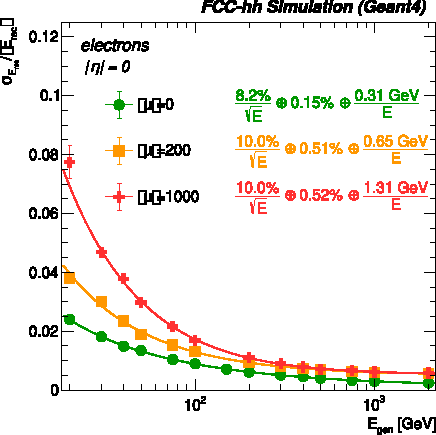
\includegraphics[width=.6\linewidth]{figures/FCC_hh_LAr_electron_performance_mu.pdf}
      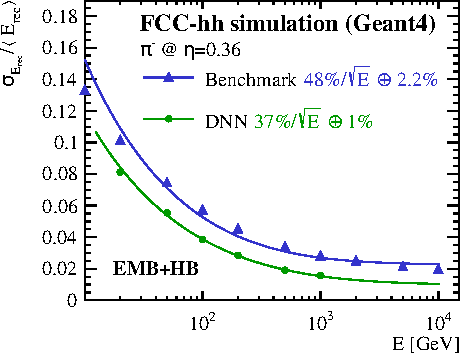
\includegraphics[width=.6\linewidth]{figures/FCC_hh_LAr_pion_performance.pdf}
    \end{center}
  \end{columns}
\end{frame}


%
% -----------------------------------------------------------------------------
%
\section{Other Calorimeter Types}

\begin{frame}
  \frametitle{CALICE}

  Collaboration of mostly Si/Tungsten based high granularity calorimeters\\[1ex]
  \bluetext{Traits:}
  \begin{columns}[c]
    \column{.4\textwidth}
    \begin{itemize}
      \item Large area silicon detectors
      \item Si Photomultipliers
      \item Highly integrated front-end electronics with timing
      \item Very large number of channels
    \end{itemize}

    \column{.6\textwidth}
    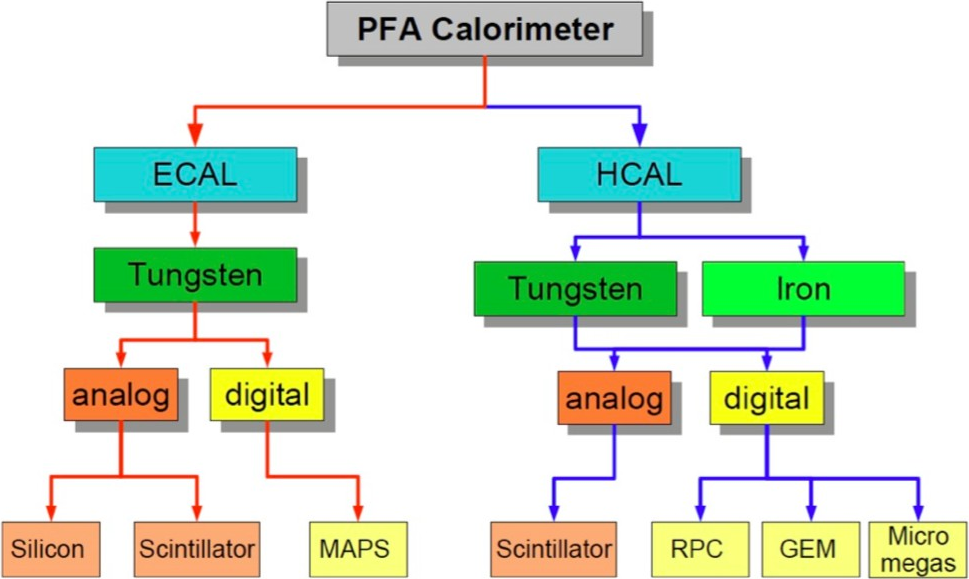
\includegraphics[width=\linewidth]{figures/CALICE_diagram.png}
  \end{columns}
\end{frame}


\begin{frame}
  \frametitle{FCC-ee: CLD Calorimeter}

  \bluetext{CLD proposal:}
  \begin{itemize}
    \item 40 layers SiW ECAL (22 $X_0$)
    \item 60 layers Scint/Steel HCAL (7.5 $\lambda_\text{I}$ +
          1 $\lambda_\text{I}$ in ECAL)
  \end{itemize}

  \begin{center}
    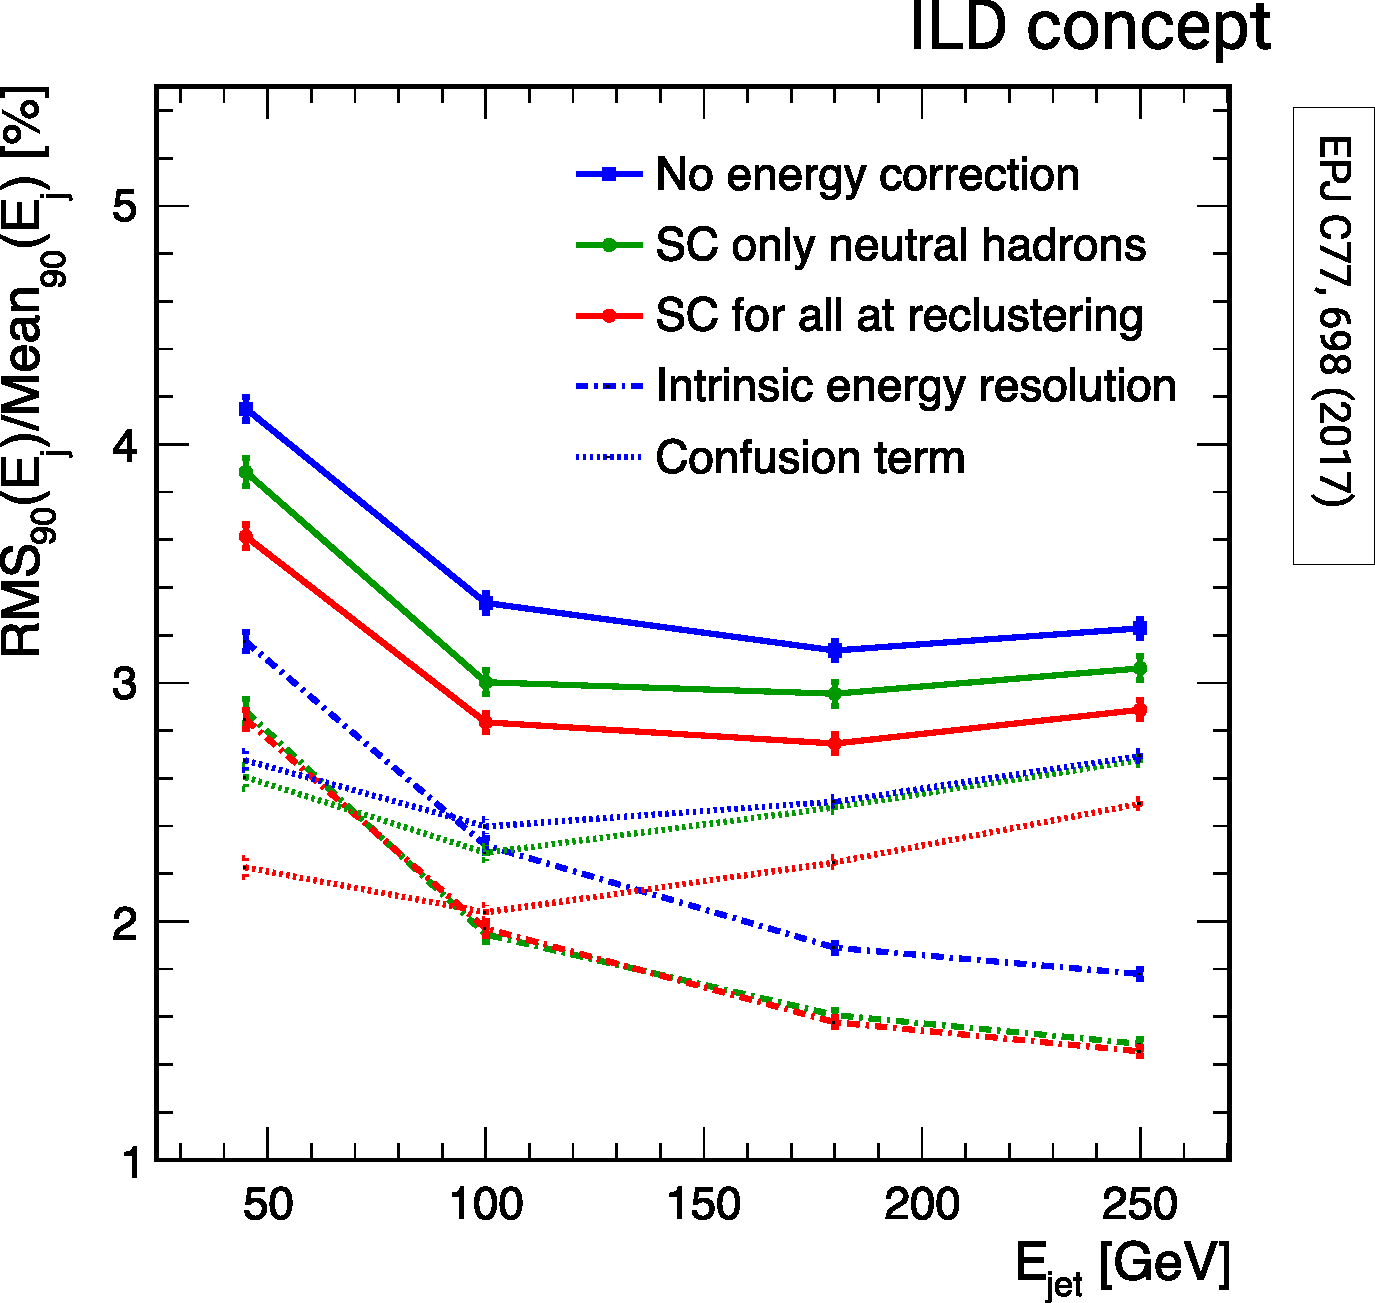
\includegraphics[width=0.41\linewidth]{figures/CLD_jet_performance.pdf}
    \hspace{7mm}
    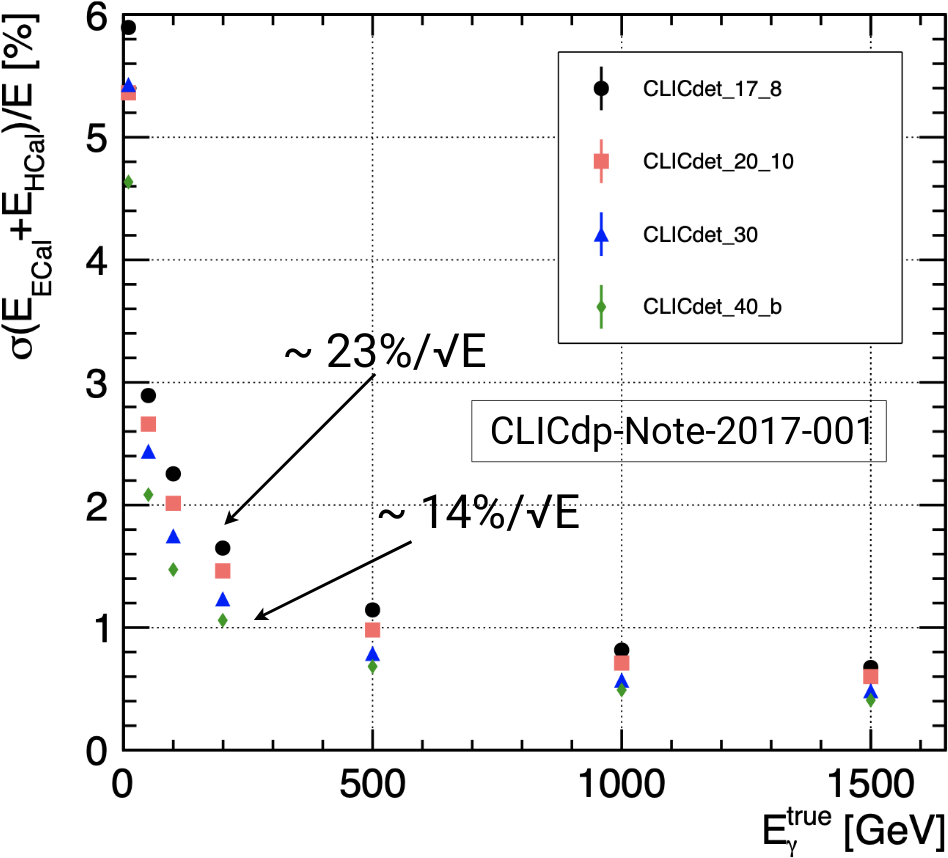
\includegraphics[width=0.41\linewidth]{figures/CLD_photon_performance.png}
  \end{center}
\end{frame}


\begin{frame}
  \frametitle{FCC-ee: IDEA Calorimeter}

  \bluetext{Traits:}
  \begin{itemize}
    \item Dual readout calorimeter with 1.5~mm pitch between
          Cherenkov and Scintillation fibers
    \item Single EM + HAD sampling calorimeter
    \item No mechanical longitudinal segmentation ($\sim 7 \lambda_\text{I}$)
    \item Good EM intrinsic energy resolution
    \item Excellent hadronic resolution
  \end{itemize}

  \vspace*{-2.1ex}
  \begin{center}
    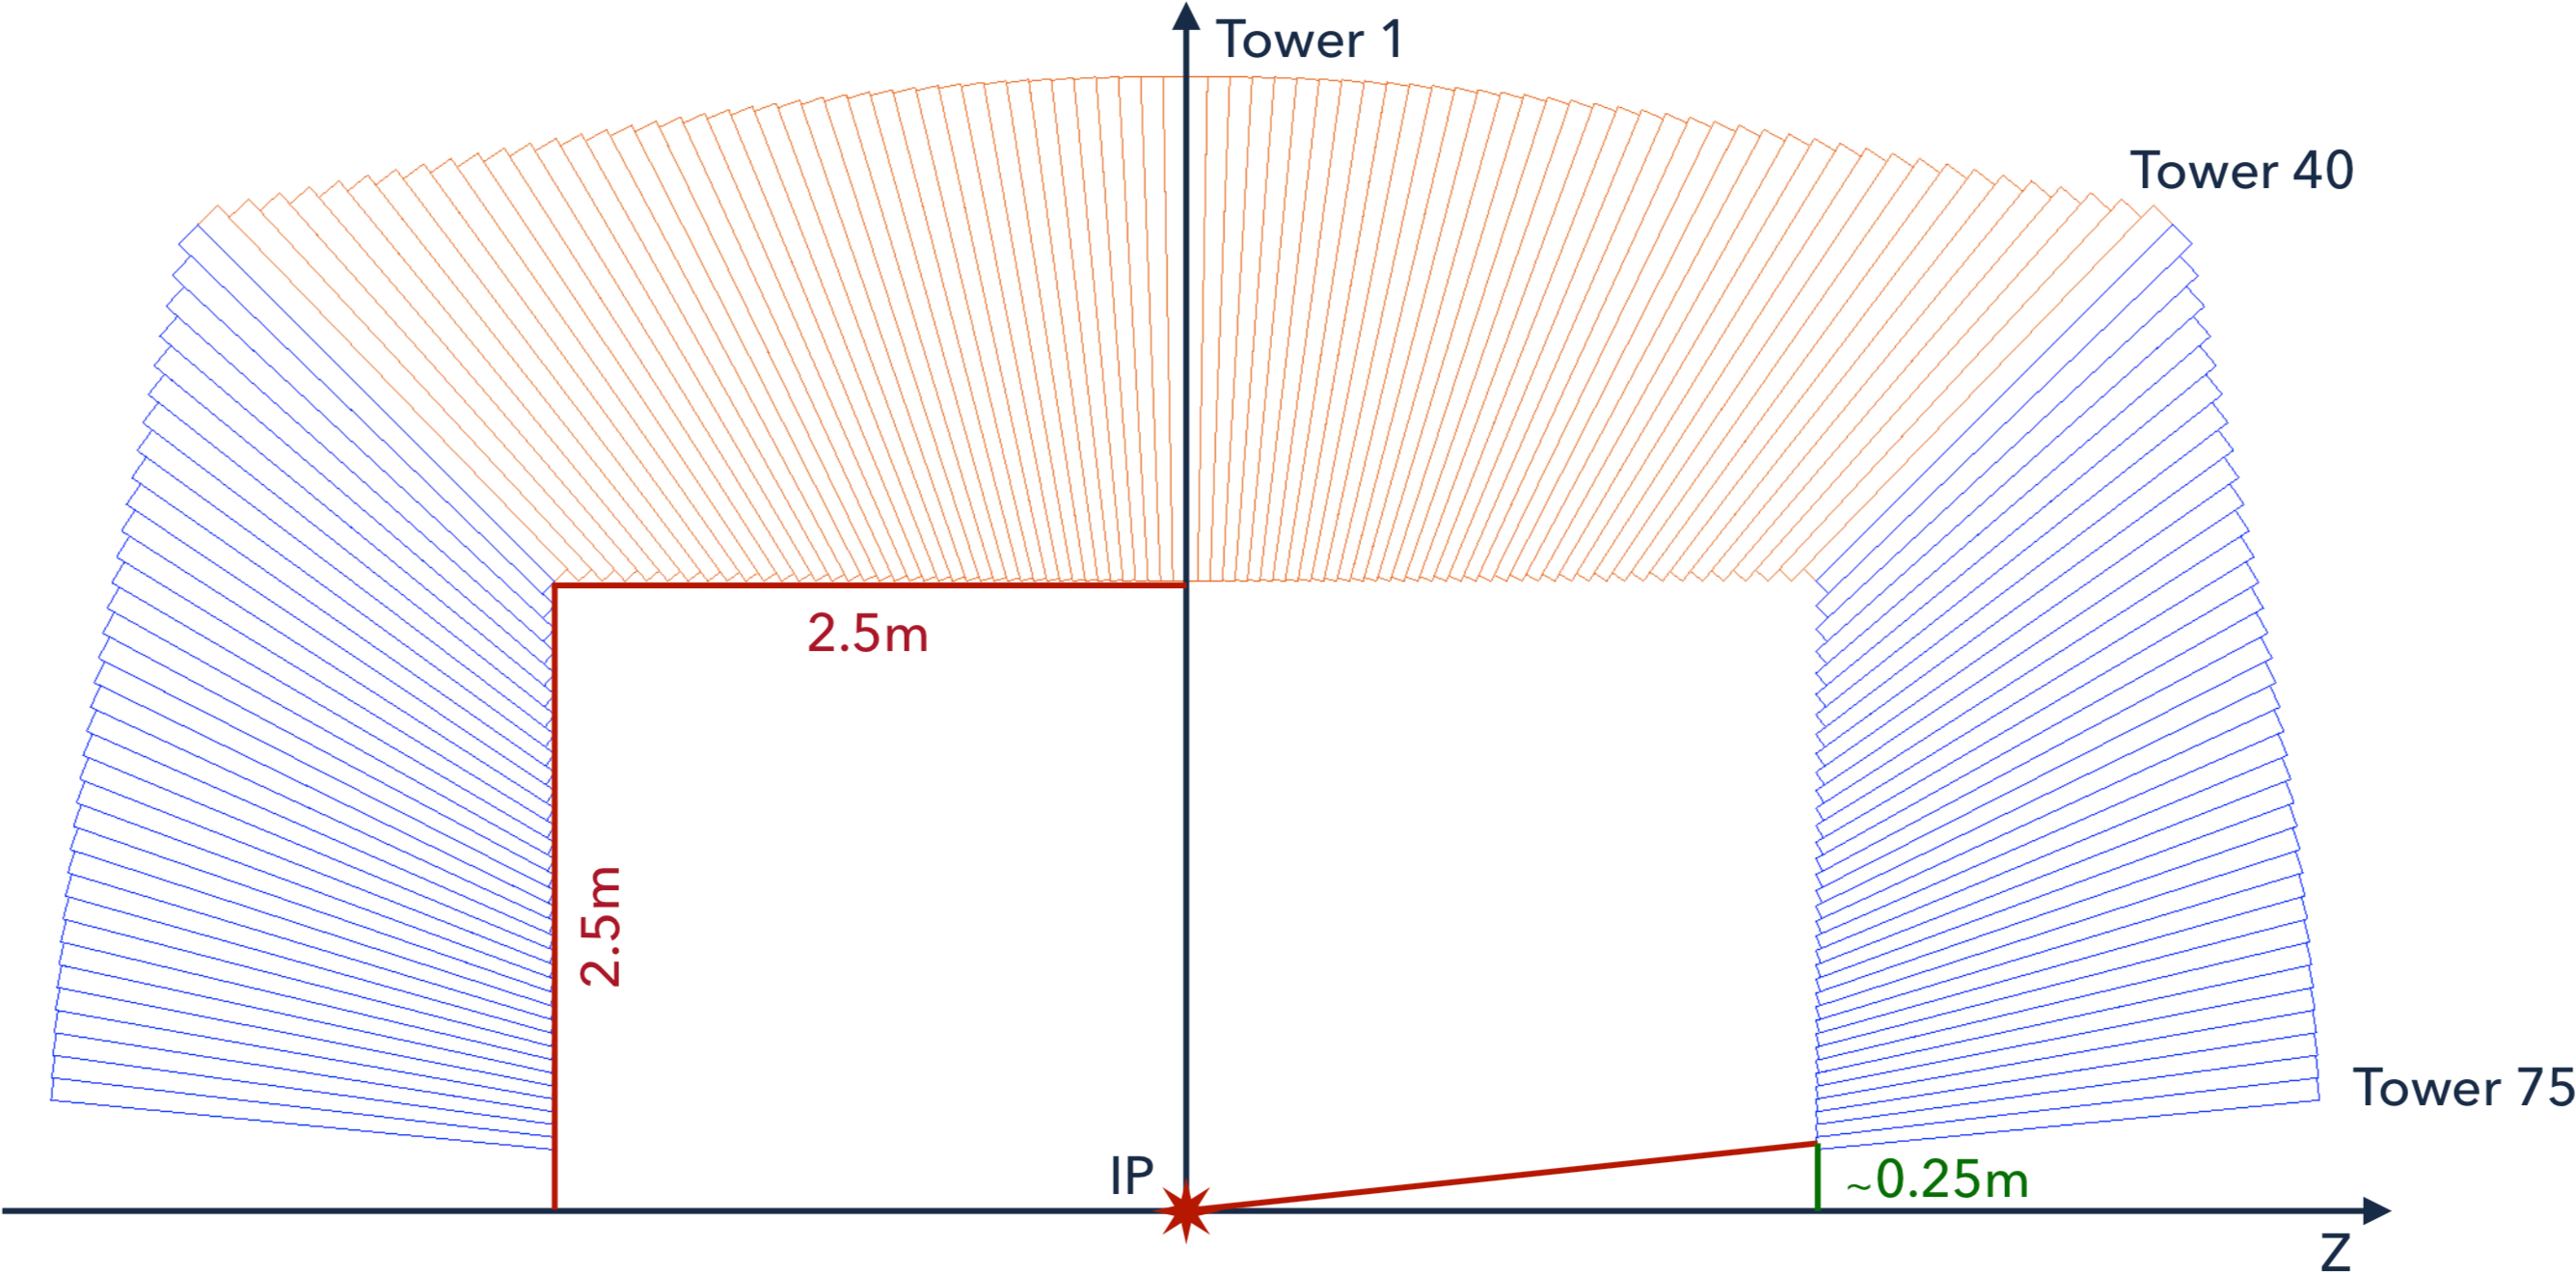
\includegraphics[width=.52\linewidth]{figures/IDEA_calorimeter_flatview.png}
  \end{center}
\end{frame}


\begin{frame}
  \frametitle{Dual Readout Calorimeter}

  \begin{columns}[c]
    \column{.5\textwidth}
    \bluetext{Principle:}
    \begin{itemize}
      \item Correct $f_\text{em}$ in every event
            \begin{itemize}
              \item Main source of fluctuations
            \end{itemize}
      \item Fibers pointing toward IP
            \begin{itemize}
              \item \bluetext{Scintillating:} sense charged
              \item \bluetext{Clear:} sense Cherenkov, mostly electrons
            \end{itemize}
    \end{itemize}

    \column{.5\textwidth}
    \begin{center}
      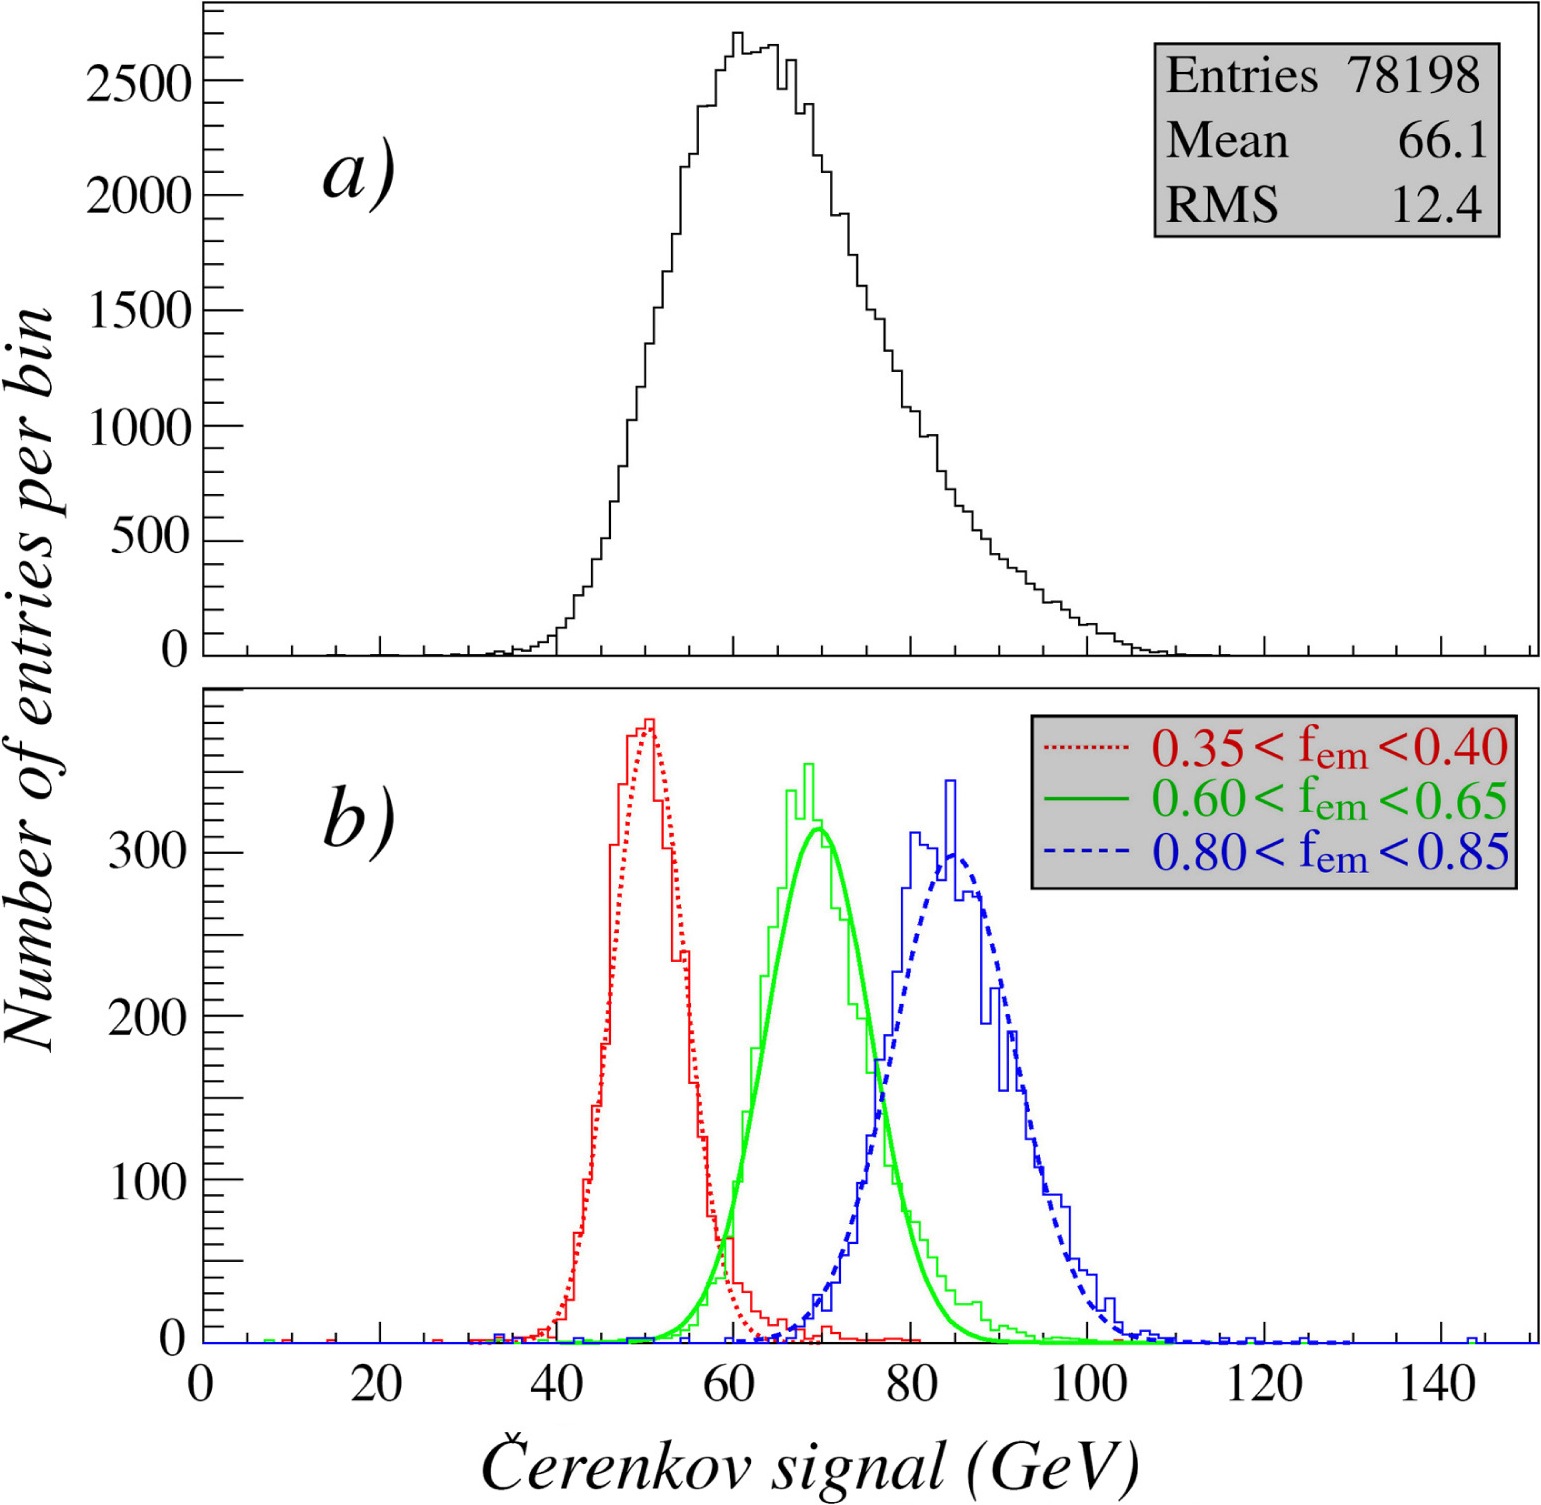
\includegraphics[width=.8\linewidth]{figures/dual_readout_signal_example.png}
      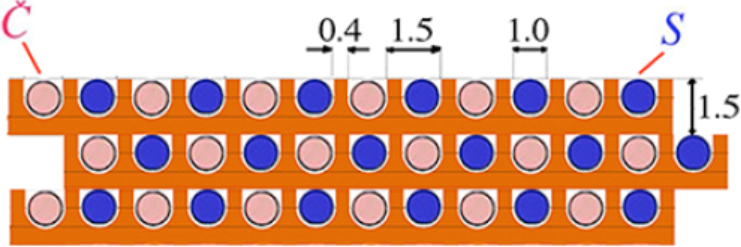
\includegraphics[width=.8\linewidth]{figures/IDEA_calorimeter_fibers.png}
    \end{center}
  \end{columns}
\end{frame}


\begin{frame}
  \frametitle{Crystal Calorimeters}

  \begin{columns}[c]
    \column{.5\textwidth}
    \bluetext{Traits:}
    \begin{itemize}
      \item Mostly investigated for CEPC
      \item Used by CMS
      \item Homogeneous structure
      \item Has optimal intrinsic energy resolution:
            $\sim 3\%/\sqrt{E\,} \, \oplus \sim 1\%$
    \end{itemize}

    \column{.5\textwidth}
    \begin{center}
      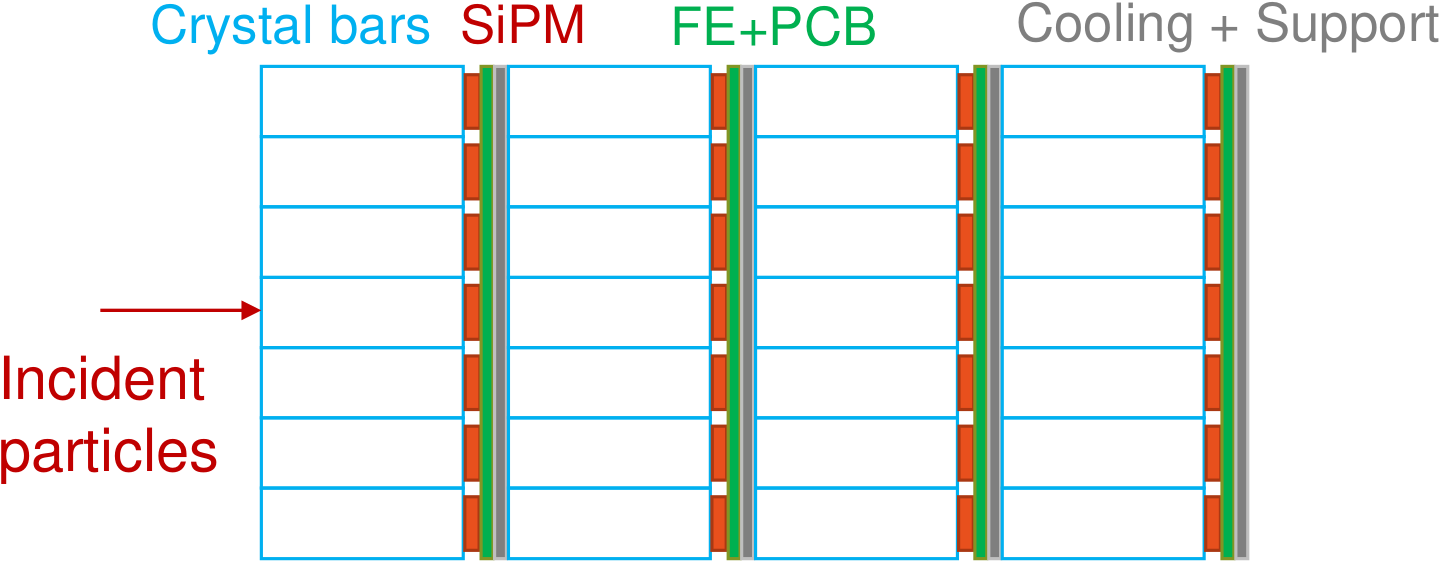
\includegraphics[width=\linewidth]{figures/CEPC_crystal_calo_design1.png}%
      \vspace{2ex}
      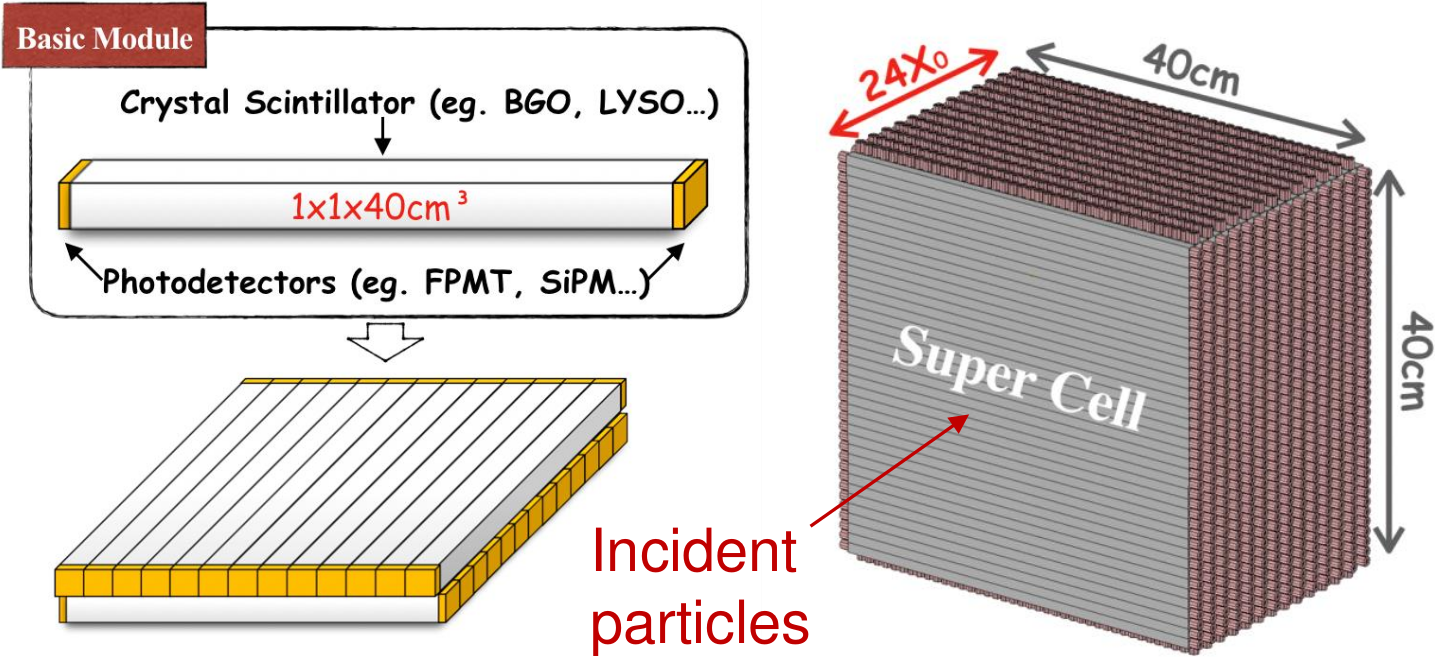
\includegraphics[width=\linewidth]{figures/CEPC_crystal_calo_design2.png}
    \end{center}
  \end{columns}
\end{frame}


%
% -----------------------------------------------------------------------------
%
\section{Improvements in Noble-liquid for FCC-ee}

\begin{frame}
  \frametitle{Improvements in Noble Liquid Calorimetry}

  \begin{itemize}
    \item Noble liquid is viable technology for FCC-ee detectors
    \item New round of optimizations started with multiple R\&D projects
    \item Both hardware and software improvements are required to get to 3\%
    \item Design driven by Particle Flow
  \end{itemize}

  \vspace{-1.5em}
  \begin{center}
    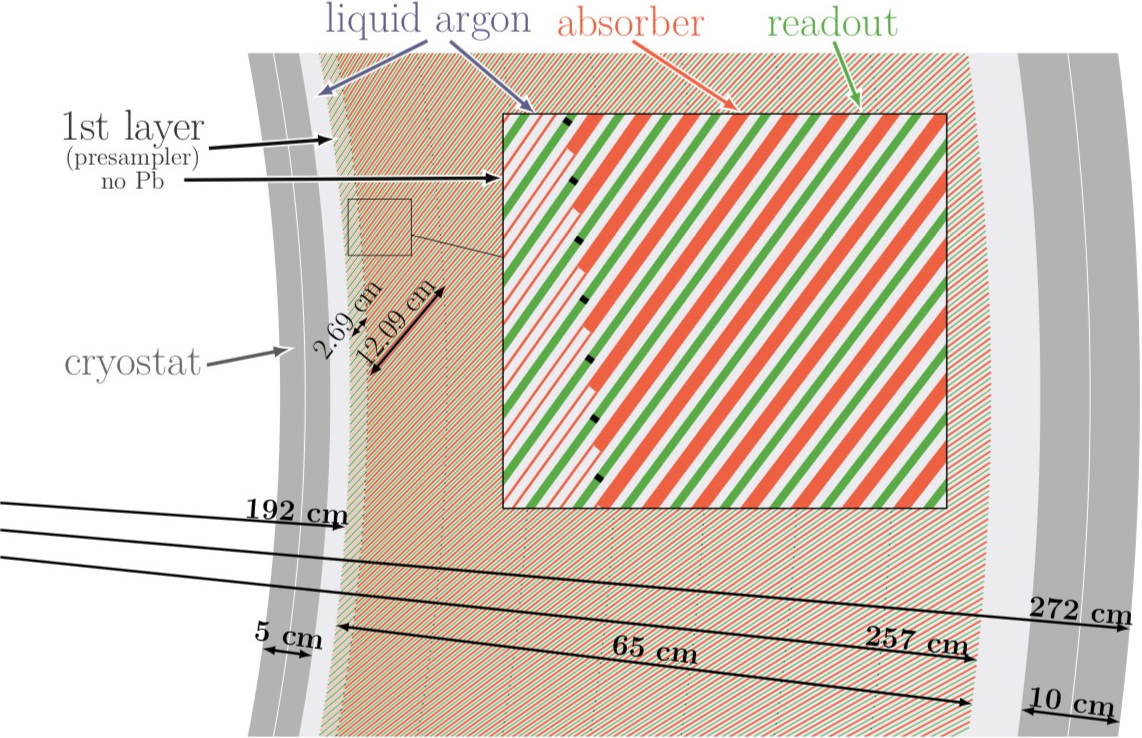
\includegraphics[align=c,width=0.47\linewidth]{figures/FCC_hh_LAr_diagram.png}%
    \hfill
    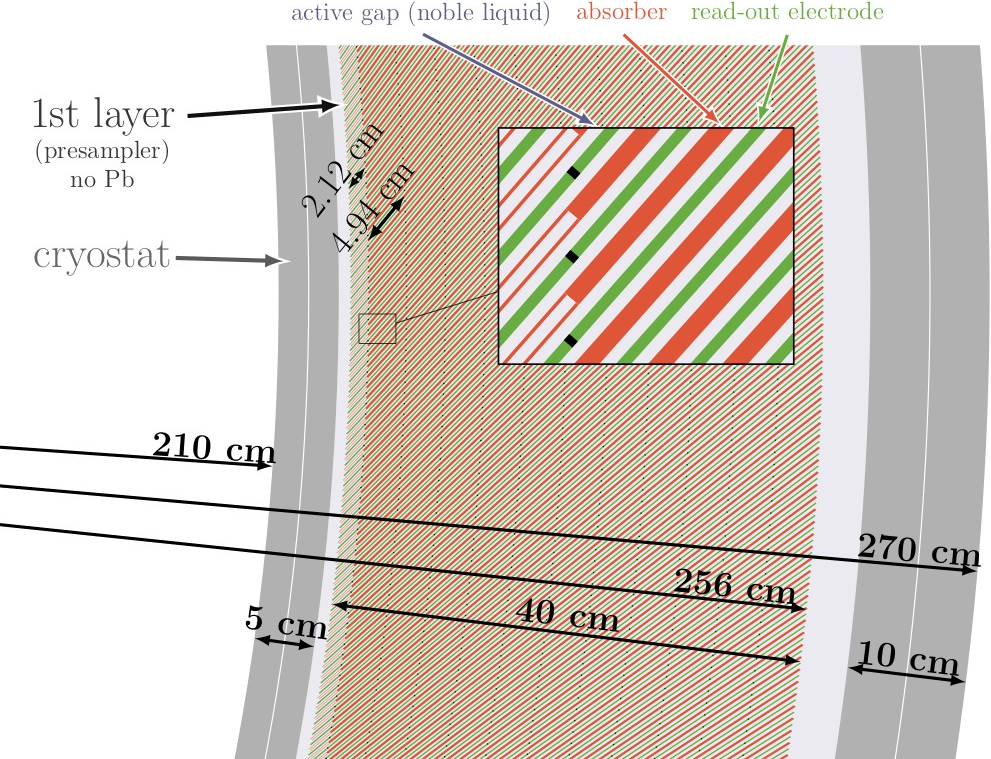
\includegraphics[align=c,width=0.47\linewidth]{figures/FCC_ee_LAr_diagram.png}\\[.5em]
    FCC-hh \hspace{16em} FCC-ee
  \end{center}
\end{frame}


\begin{frame}
  \frametitle{Particle Flow}

  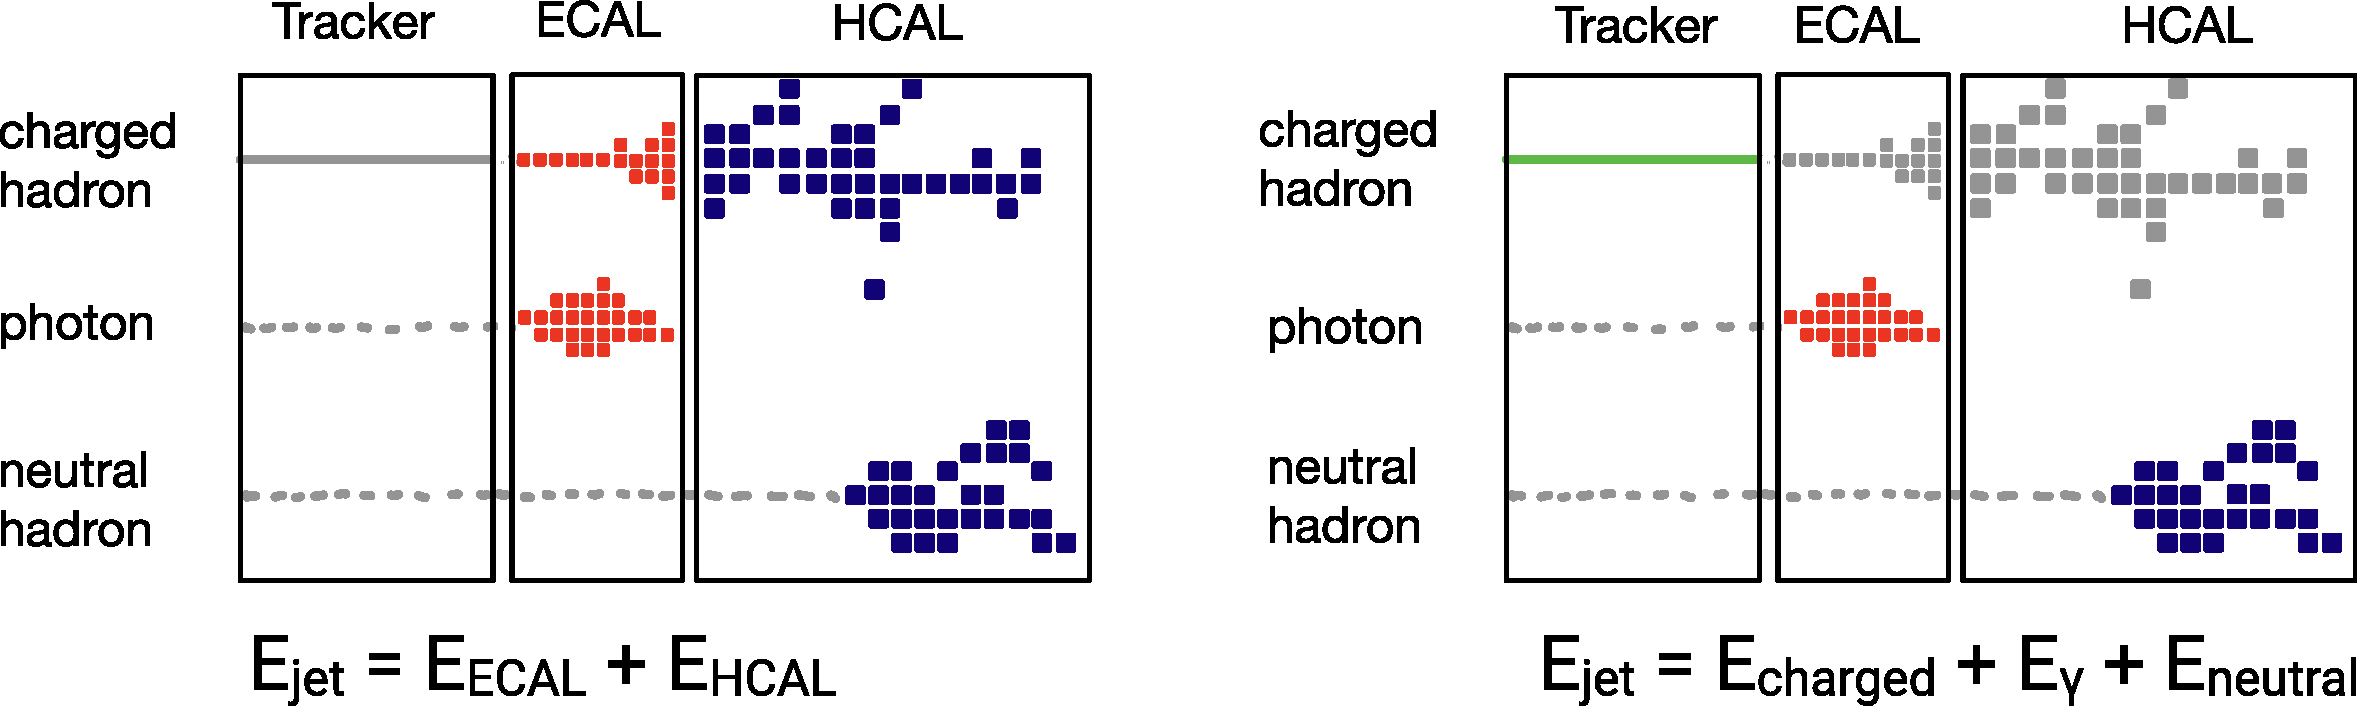
\includegraphics[width=\linewidth]{figures/particle_flow_diagram.pdf}
  \vspace{-1.5ex}
  \hspace{6.7em} 30\% + 70\% \hspace{14.5em} 60\% + 30\% + 10\%

  \vspace{-1ex}
  \bluetext{Idea:}
  \begin{columns}[c]
    \column{.5\textwidth}
    \begin{itemize}
      \item Reconstruct every particle in the event with the best possible
            precision
      \item Combine the measurements in subdetectors in an optimal way
    \end{itemize}

    \column{.5\textwidth}
    \begin{itemize}
      \item Charged particles dominated by tracker
      \item Calorimetry mostly for neutral particles
      \item \bluetext{Enemy: Confusion}
    \end{itemize}
  \end{columns}

\end{frame}

\begin{frame}
  \frametitle{Hardware Improvements}

  \begin{columns}[c]
    \column{.5\textwidth}
    \begin{itemize}
      \item Tested technology in ATLAS
      \item Less than $10\%/\sqrt{E}$ demonstrated
    \end{itemize}

    \bluetext{Improvements for FCC-ee}
    \begin{itemize}
      \item Higher granularity
            \begin{itemize}
              \item Transverse and in depth
              \item More signal traces
            \end{itemize}
      \item Improve EM resolution
            \begin{itemize}
              \item Higher sampling fraction $\rightarrow$ thicker detector
            \end{itemize}
      \item Low energy photons \\
            (bellow 300 MeV)
            \begin{itemize}
              \item Low mass cryostat
              \item Smaller noise term
            \end{itemize}
    \end{itemize}

    \column{.5\textwidth}
    \begin{center}
      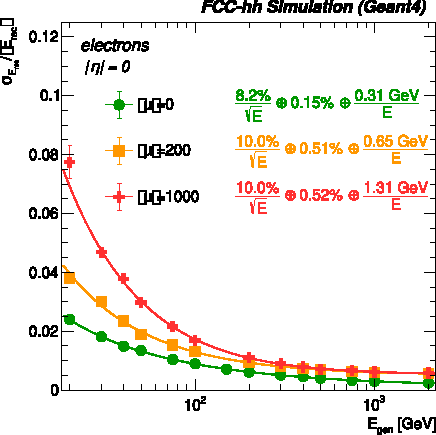
\includegraphics[width=.6\linewidth]{figures/FCC_hh_LAr_electron_performance_mu.pdf}
      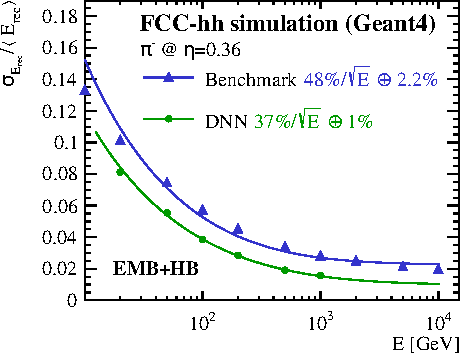
\includegraphics[width=.6\linewidth]{figures/FCC_hh_LAr_pion_performance.pdf}
    \end{center}
  \end{columns}
\end{frame}


\begin{frame}
  \frametitle{Improvements for FCC-ee}

\end{frame}


\begin{frame}
  \frametitle{Hardware Improvements for FCC-ee}

  \begin{itemize}
    \item Optimization using FCCSW will be performed
          \begin{itemize}
            \item $22 X_0$, $7\lambda_\text{I}$ sufficient
            \item Granularity, sampling frequency, sampling fraction
            \item Active material (Krypton, \dots)
            \item Absorber material (Tungsten, \dots)
          \end{itemize}
  \end{itemize}

  \begin{itemize}
    \item High density feedthroughs for signal out of the calorimeter
    \item High granularity electrodes
    \item Detector geometry
    \item Minimizing material budget
    \item High rate mitigation
  \end{itemize}
\end{frame}

\begin{frame}
  \frametitle{Software Improvements for FCC-ee}

  \begin{columns}[c]
    \column{.6\textwidth}
    \begin{itemize}
      \item New generic framework Key4HEP emerges from the FCCSW and iLCSoft
      \item Based on Gaudí but uses Podio
      \item Integrates tools from simulation, detector description to
            reconstruction
      \item Integration of Particle Flow algorithm (Pandora SDK)
      \item Reimplementation of clustering algorithm (CLUE)
      \item Replacement of ECal in CLD or IDEA by LAr calorimeter
    \end{itemize}

    \column{.4\textwidth}
    \begin{center}
      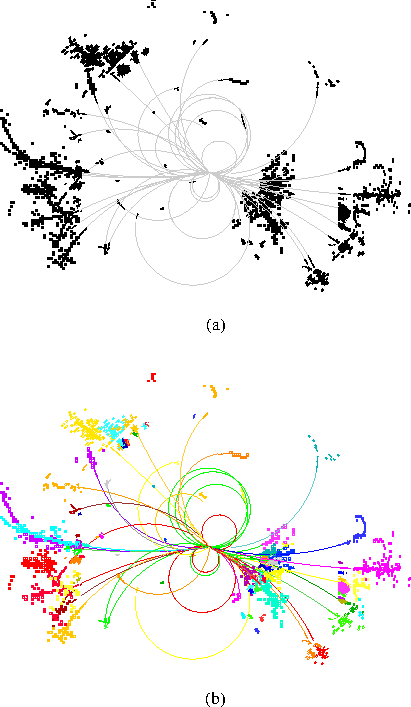
\includegraphics[width=.7\linewidth]{figures/pandora_example.pdf}
    \end{center}
  \end{columns}
\end{frame}

%
% -----------------------------------------------------------------------------
%
\section{Conclusions and Plans}

\begin{frame}
  \frametitle{Conclusion and Plans}

  \begin{itemize}
    \item LAr calorimeters were investigated mostly for FCC-hh
    \item Investigate LAr performance in the FCC-ee framework
          \begin{itemize}
            \item Replace existing CLD/IDEA calorimeters with LAr
          \end{itemize}
    \item Implement particle flow algorithm for LAr calorimeter
    \item Multiple R\&D projects directed at LAr at FCC-ee
  \end{itemize}
\end{frame}

%
% -----------------------------------------------------------------------------
%
\appendix
\backupbegin{}

\begin{frame}[c]
  \begin{center}
    \redtext{\Huge Backup}
  \end{center}
\end{frame}


\begin{frame}
  \frametitle{R\&D FCC-ee LAr Projects}

  CERN EP R\&D projects relevant for Noble Liquid Calorimetry:

  \begin{enumerate}
    \item Read-Out Electrode Design and Performance Optimization
    \item High Density Feed Through Design Investigations
    \item Carbon Composite Cryostats
    \item General SW framework
  \end{enumerate}

  CERN, Charles U. and LAL Orsay: H2020 project AIDAInnova

\end{frame}


\begin{frame}
  \frametitle{Dual Readout Performance}

  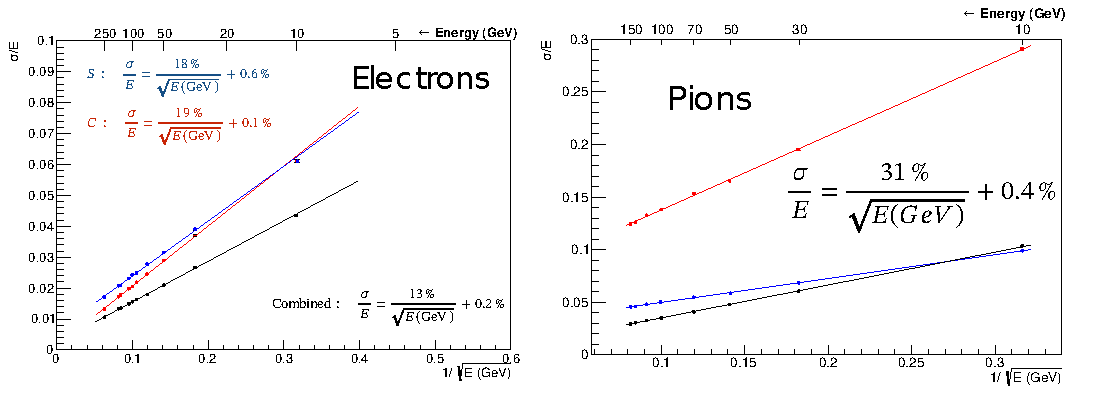
\includegraphics[width=\linewidth]{figures/dual_readout_performance.pdf}
\end{frame}

\begin{frame}
  \frametitle{Crystals Performance}

  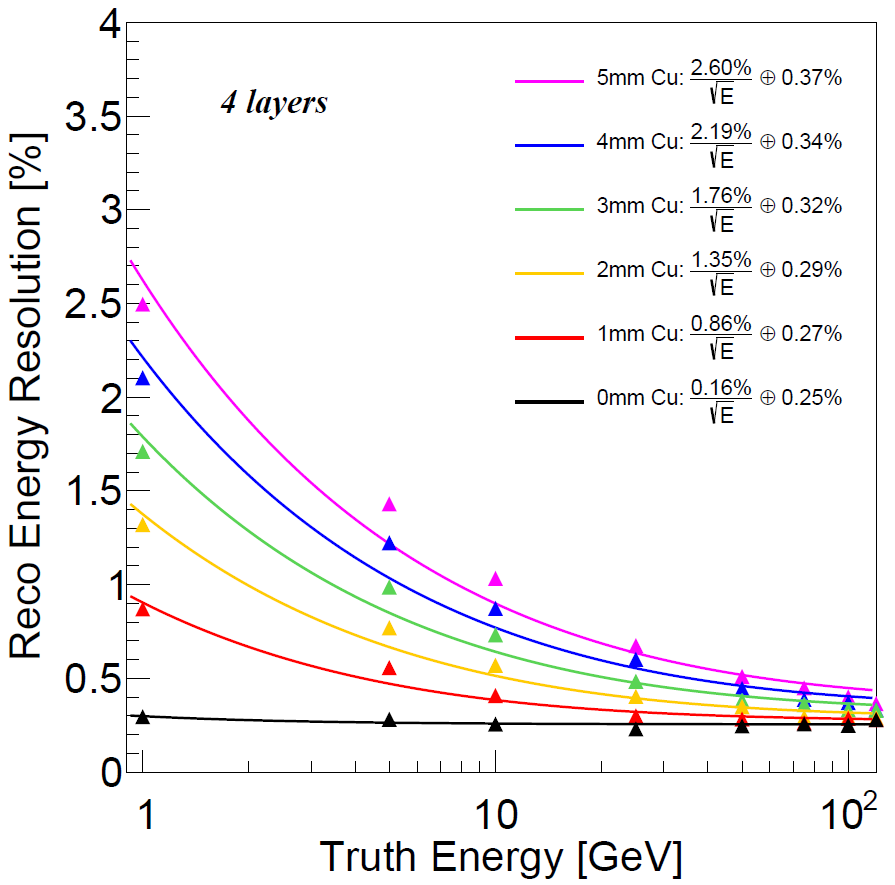
\includegraphics[width=.49\linewidth]{figures/CEPC_crystal_calo_perf_4layers.png}
  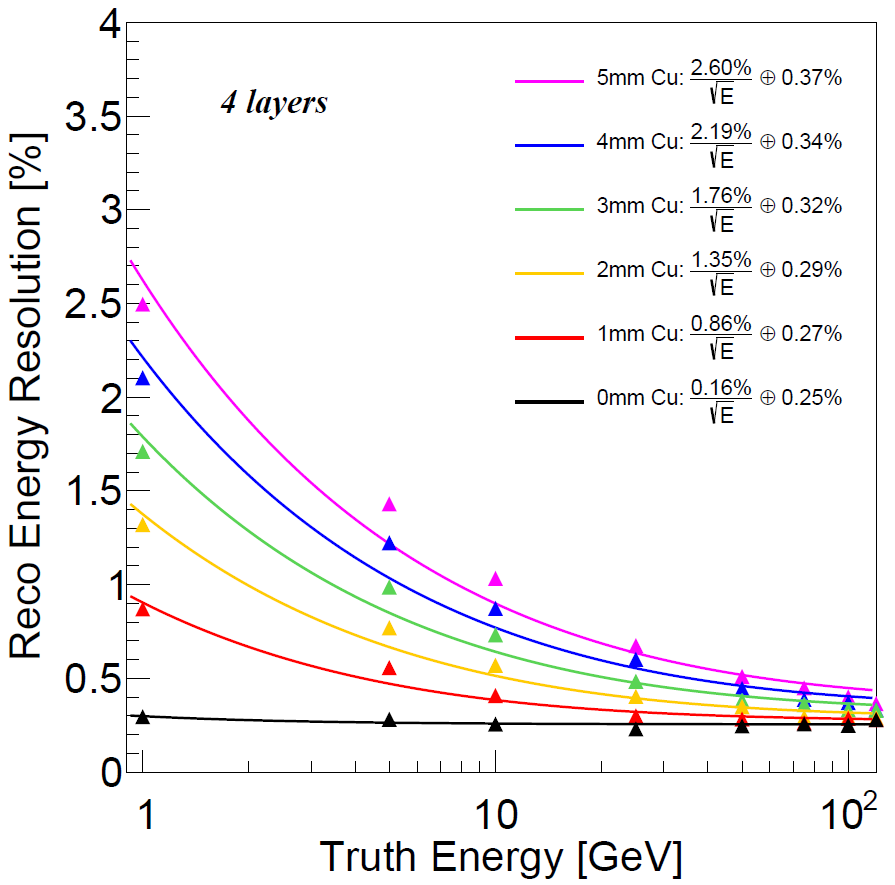
\includegraphics[width=.49\linewidth]{figures/CEPC_crystal_calo_perf_4layers.png}
\end{frame}


\begin{frame}
  \frametitle{FCC-hh: Reference Detector}

  \begin{adjustwidth}{-2em}{-2em}
    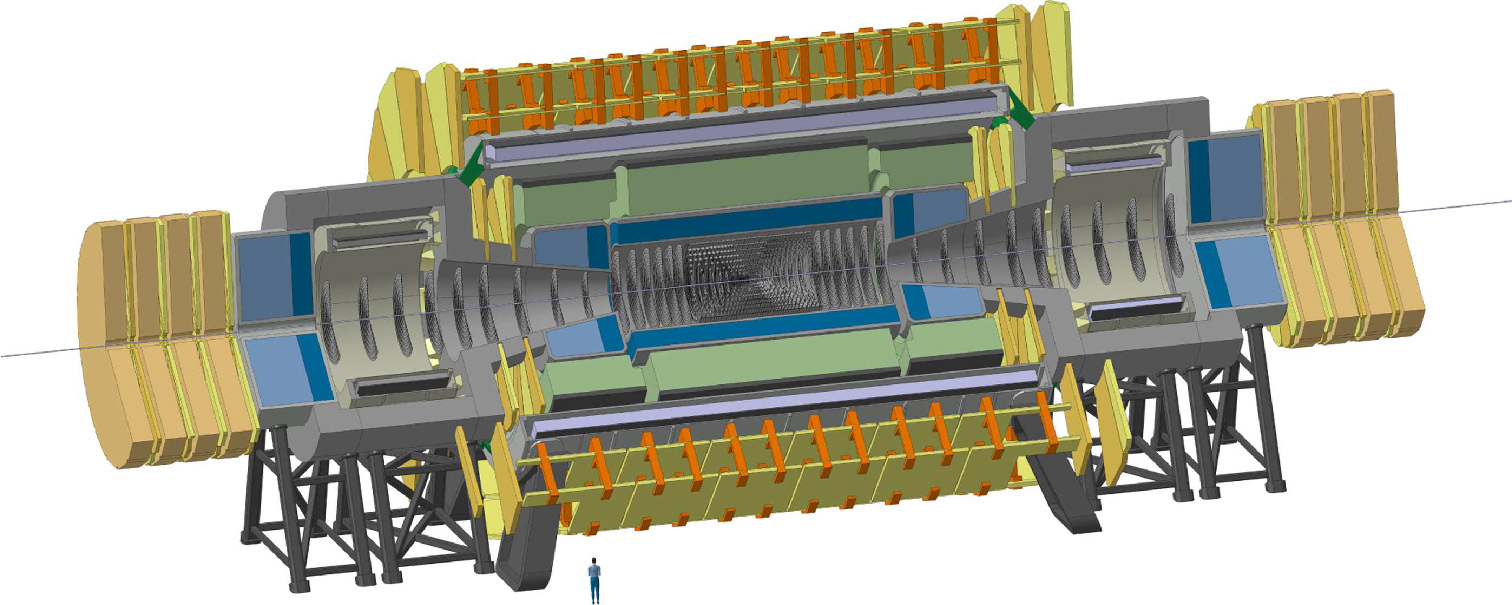
\includegraphics[width=\linewidth]{figures/FCC_hh_ref_detector.png}
  \end{adjustwidth}
\end{frame}

\begin{frame}
  \frametitle{FCC-hh: Reference Detector}

  \begin{adjustwidth}{-2em}{-2em}
    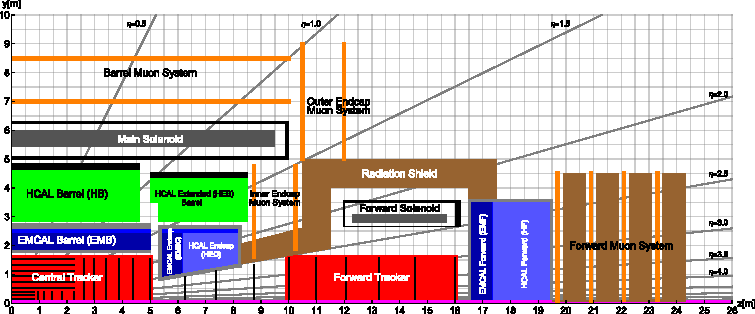
\includegraphics[width=\linewidth]{figures/FCC_hh_ref_detector_xsec.pdf}
  \end{adjustwidth}
\end{frame}

\backupend{}

\end{document}
